\documentclass[12pt, a4paper]{article}
\edef\restoreparindent{\parindent=\the\parindent\relax}
\usepackage{amsmath}
\usepackage[UKenglish]{babel}
\usepackage[bibstyle=ieee, dashed=false, sorting=nty]{biblatex}
\usepackage[labelfont=bf]{caption}
\usepackage{colortbl}
\usepackage{csquotes}
\usepackage{fancyhdr}
\usepackage{float}
\usepackage[top=25mm, right=25mm, bottom=25mm, left=25mm]{geometry}
\usepackage{graphicx}
\usepackage{hyperref}
\usepackage[capitalise, nameinlink, noabbrev]{cleveref}
\usepackage{listings}
\usepackage{longtable}
\usepackage{minted}
\usepackage{microtype}
\usepackage{multirow,multicol}
\usepackage{parskip}
\usepackage{tikz, pgfplots}
\usepackage{tcolorbox}
\usepackage{textcomp} % for trademark, copyright symbol
\usepackage{xcolor}

\restoreparindent

\pagestyle{fancy}
\fancyhead[L]{COM4521}
\fancyhead[C]{Assignment: N-body Simulation}
\fancyhead[R]{Part 1}
\setlength{\headheight}{15pt}

\usemintedstyle{vs}

% colours used in table
\definecolor{lightgray}{HTML}{E3E3E3}
\definecolor{green}{HTML}{B7E1CD}

\pgfplotsset{compat=newest}
\usepgfplotslibrary{units}
\usepgfplotslibrary{groupplots}

\let\oldcref\cref
\renewcommand{\cref}[1]{\textbf{\oldcref{#1}}}

\addbibresource{references.bib}

\begin{document}

\renewcommand{\baselinestretch}{1.3}\normalsize
\tableofcontents
\renewcommand{\baselinestretch}{1.0}\normalsize
\newpage

\section{Pre-Implementation Considerations}
Several aspects are considered in advance to facilitate the implementation process and to improve
the overall programming quality.

\subsection{Programming Practices} \label{sec:practices}
To minimise the risk of programming pitfalls, a set of good practices is adopted. These practices
are assessed according to their relative importance to the quality. Below is the list of practices
ordered in descending importance level.

\begin{enumerate}
  \item \textbf{Robustness:} The program must be able to handle any user input without crashing. If
  a given input is invalid, the program should return a descriptive error message.
  \item \textbf{Maintainability:} Follow a consistent coding style and use the self-documenting
  function and variable names. Refactor the code so that each function is only responsible for one
  task. Code with good structure and high cohesion will be able to narrow down the range of
  potential problems in the future.
  \item \textbf{Computational Resource Efficient:} Perform the minimum amount of computation in a
  loop if possible. Minimise overhead by reducing the number of function calls in a loop. If the
  value of a computationally expensive operation will be used multiple times, then store it into a
  variable.
  \item \textbf{Documentation:} The code should be well commented. Each function should have a
  Javadoc style block comment before the function definition. It is preferred to write
  self-documenting code, however, inline comments should be used when further clarification is
  required.
\end{enumerate}

\subsection{Unit Testing}
Since the program involves user input processing, thus it is required to perform basic unit testing
to test its correctness and completeness in handling user inputs.

It is impractical to test every possible combination of user inputs. Therefore, each command
argument will be tested independently with their respective edge cases. Testing the program with
edge cases is an efficient way to ensure that the problem can handle extreme user inputs.

\begin{table}[H]
  \centering
  \begin{tabular}{|c|c|c|c|}
    \hline \rowcolor{lightgray}
    Test Case & Argument & Expected Result & Status \\ \hline
    & & & \\ \hline
    \end{tabular}
  \caption{Documentation format of unit testing.}
\end{table}

\subsubsection{Limitations}
Unit testing with edge cases will not catch every error in the program, such as runtime errors or
system-level errors. It is possible for the program to produce incorrect behaviour while passing all
the test cases. To mitigate this issue, the number of benchmarks has to be increased to reduce the
likelihood of unexpected errors.

\section{Preliminary Tasks Implementation}
This section discusses and compares the various possible techniques for implementing the preliminary
tasks before the N-body simulation.

\subsection{Arguments Processing}
\subsubsection{Integer Arguments} \label{subsec:args}
\begin{tcolorbox}
\textbf{Problem:} The integer arguments (\textbf{N}, \textbf{D}, and \textbf{I}) are saved as
`string' in \mintinline{c}{char *argv[]}.

\bigskip\textbf{Goal:} Parse and convert the `string' into \mintinline{c}{unsigned int} (the same
data type used in \mintinline{c}{NBodyVisualiser.c}).
\end{tcolorbox}

Each input argument \textbf{N}, \textbf{D}, and \textbf{I} can be categorised as follows:
\begin{enumerate}
  \item \textbf{Category 1:} Argument is a string (e.g. "abc"). In this case, the program must
  exit with an error message since the argument is not a valid integer and cannot be converted.
  \item \textbf{Category 2:} Argument is a negative number. Since the data type will be
  \mintinline{c}{unsigned int}, the program must exit with an error message.
  \item \textbf{Category 3:} Argument is zero. For \textbf{N} and \textbf{D}, the value must be
  larger than 1 so the program will exit with an error message. For \textbf{I}, the program will
  accept the argument but start in \textbf{visualisation} mode.
  \item \textbf{Category 4:} Argument is a positive number. In this category, there are two more
  cases to be considered:
  \begin{enumerate}
    \item argument $\leq$ \mintinline{c}{INT_MAX}. The program should accept the argument and
    produce no error. If the number is very large and the machine has limited computational
    resources, then the program will either return a memory allocation error (discussed in
    \cref{sec:malloc}) before the simulation or encounter errors including out-of-memory error,
    system not responding error, etc. during the simulation.
    \item argument $>$ \mintinline{c}{INT_MAX}. The is the case where overflow occurs. The program
    should return an error and exit.
  \end{enumerate}
\end{enumerate}

\textcolor{red}{N.B.} Changes are made to the definition of \textbf{Category 4} in the second
iteration. Refer to \cref{subsec:c3016} for detailed explanation.

Based on the analysis of input categorisation, the problem is now clearly defined and the
implementation approach can be chosen. The C standard library \mintinline{c}{stdlib.h} provides
different functions that can convert a string to different integer types. Firstly, the
implementation has to choose a function with appropriate return type. However, there are several
return types that are not suitable for the use case, as justified below:
\begin{enumerate}
  \item A function with return type of \mintinline{c}{int} is not able to satisfy the conditions in
  \textbf{Category 4}. Argument inputs that are larger than \mintinline{c}{INT_MAX} will cause
  overflow of \mintinline{c}{int}.

  \item According to the official Microsoft documentation on storage of basic types
  \cite{basic_types_storage}, \mintinline{c}{long} has the same storage size as \mintinline{c}{int}
  (4 bytes). Therefore, it will have the same issue as (1).

  \item Function that returns \mintinline{c}{float}, \mintinline{c}{double}, or \mintinline{c}{long
  double} are not suitable as they are primarily use for floating point numbers.
\end{enumerate}

After applying these restrictions, the available functions for selection are:
\begin{itemize}
  \item \mintinline{c}{atoll}: returns \mintinline{c}{long long int}
  \item \mintinline{c}{strtoll}: returns \mintinline{c}{long long int}
  \item \mintinline{c}{strtoul}: returns \mintinline{c}{unsigned long int}
  \item \mintinline{c}{strtoull}: returns \mintinline{c}{unsigned long long int}
\end{itemize}

\subsubsection*{Conclusion}
\mintinline{c}{strtoul} is chosen to be the function for integer arguments processing. This is
because:
\begin{enumerate}
  \item Its return type is \mintinline{c}{unsigned long int}, which has the same size and range as
  \mintinline{c}{unsigned int} \cite{basic_types_storage}. In comparison with a \mintinline{c}{long
  long} type, it would use less computational resources and this comply with \textbf{Programming
  Practice 3}.
  \item It stops reading the string at the first character it cannot recognize as part of a number
  \cite{strtoul}. This is helpful for error checking the string.
\end{enumerate}


\subsubsection{Operation Mode (M)}
There are only two valid enum values for the operation mode: \mintinline{c}{CPU} and
\mintinline{c}{OPENMP}. The program uses \mintinline{c}{strcmp()} to compare the argument
\textbf{M} with the strings \mintinline{c}{"CPU"} and \mintinline{c}{"OPENMP"}, and assign the
operation mode to the corresponding enum value.

The program will return an error message and exit if the argument \textbf{M} is other value.

\subsubsection{Input File}
The file name is stored into \mintinline{c}{char *} variable and the file content is processed in
N-body data initialisation stage later.

The program will return an error message if the option \mintinline{bash}{-f} is specified but no
file name is provided.

\subsection{N-Body Data Initialisation}
\begin{listing}[ht]
  \begin{minted}[frame=lines, framesep=2mm]{c}
  #define DEFAULT_X ((float)rand() / RAND_MAX)
  #define DEFAULT_Y ((float)rand() / RAND_MAX)
  #define DEFAULT_VX 0
  #define DEFAULT_VY 0
  #define DEFAULT_M (1 / (float)N)
  \end{minted}
  \caption{Default value of each n-body member variable} \label{listing:default}
\end{listing}

Macros are defined for the default value of each n-body member variable. They will be used for
generating random data and setting the unspecified variables in an input file.

\subsubsection{Generating Random Data}
Generating random data is straightforward. The value of each member variable is set to the
corresponding macro.

\subsubsection{Processing Input File}
\begin{tcolorbox}
\textbf{Problem:} The input file contains lines of comma separated values, each representing the
initial states of an n-body. The input file may also contain comment lines.

\bigskip\textbf{Goal:} Read the input file and process only non-comment lines. Default values should
be assigned for unspecified variables.
\end{tcolorbox}

\subsubsection*{Step 1: Reading the lines}
Each line in the input file can be categorised as follows:
\begin{enumerate}
  \item \textbf{Category 1:} The line is a comment line
  \item \textbf{Category 2:} The line is an empty line
  \item \textbf{Category 3:} The line do not have the correct number of commas
  \item \textbf{Category 4:} The line contains invalid values (e.g. a string)
  \item \textbf{Category 5:} The line contains 5 values and the correct number of commas
  \item \textbf{Category 6:} The line contains unspecified values and the correct number of commas
  \item \textbf{Category 7:} The line is longer than the defined \texttt{BUFFER\_SIZE} of value 64
\end{enumerate}

Lines that belong to either \textbf{Category 5} or \textbf{Category 6} should only be read and
processed by the program. This is implemented by modifying the \mintinline{c}{readLine()} function
provided in the Lab 1 Exercise 5 solution, as shown in \cref{listing:readline}.

\begin{listing}[ht]
  \begin{minted}[linenos, frame=lines, framesep=2mm, fontsize=\footnotesize]{c}
      while ((c = (char)getc(f)) != EOF) {
          // Case 1: ignore any line starting with '#'
          // Case 2: ignore any blank line
          if (i == 0 && (c == '#' || c == '\n')) {
              while (c != '\n') {
                  c = (char)getc(f);
              }
          } else {
              ...
  \end{minted}
  \caption{Code snippet of \mintinline{c}{read_line()} function.} \label{listing:readline}
\end{listing}

For \textbf{Category 3 and 4}, a helper function is created to ensure that only 4 commas appear in a
non-comment line and all values in the line can be converted into float. The function will exit the
program with an error message if the line does not contain the correct number of commas.

\subsubsection*{Step 2: Extracting the Values}
Now each line will have exactly 4 commas. Some lines will have all 5 values and some of them will
have unspecified values. Unspecifed values will then be assigned with the default values defined in
\cref{listing:default}. Firstly, the line has to be split into a series of tokens using comma as
delimiter. Each token can then be converted into \mintinline{c}{float} using the functions provided
in C standard library.

\subsubsection*{Iteration 1}
The first attempt to split the line into tokens was using the function \mintinline{c}{strtok} in C
\mintinline{c}{string.h} library. It is works well when the line is in correct format, and there
must be a space after each comma. However, in the case where the line has consecutive commas without
space between them (e.g. \mintinline{c}{0.1f,,0.2f,,}), \mintinline{c}{strtok} would extract the
second token as \mintinline{c}{0.3f} instead of \mintinline{c}{NULL}.

After further experiments, it is confirmed that \mintinline{c}{strtok} is unable to recognise empty
tokens. Therefore, a different approach has to be adapted.

\subsubsection*{Iteration 2}
\begin{listing}[ht]
  \begin{minted}[linenos, frame=lines, framesep=2mm, fontsize=\footnotesize]{c}
  static char *tokenise(char *buffer) {
      static char *buffer_start = NULL;

      if (buffer != NULL) buffer_start = buffer;

      // see if we have reached the end of the line
      if (buffer_start == NULL || *buffer_start == '\0') return NULL;

      // return the number of characters that are not delimiters
      const unsigned int n = strcspn(buffer_start, ",");

      // return token as NULL for consecutive delimiters
      if (n == 0) {
          buffer_start += 1;
          return NULL;
      }

      // save start of this token
      char *p = buffer_start;

      // bump past the delimiters
      buffer_start += n;

      // remove the delimiters
      if (*buffer_start != '\0') *buffer_start++ = '\0';

      return p;
  }
  \end{minted}
  \caption{Code snippet of \mintinline{c}{tokenise()} function.} \label{listing:tokenise}
\end{listing}

The new approach attempts to address the problem in \textbf{Iteration 1} by creating a customised
version of \mintinline{c}{strtok} function (\cref{listing:tokenise}). Line 13 - 16 allow the
\mintinline{c}{tokenise} to return NULL as the token between two consecutive delimiters.

\subsection{Memory Allocation} \label{sec:malloc}
% use calloc instead of malloc+memset. TODO: prove by benchmark

As mentioned in \cref{subsec:args}, memory error might occur if the integer arguments \textbf{N} and
\textbf{D} are large and the machine does not have sufficient memory for dynamic allocation. This
can be avoided by having a \mintinline{c}{NULL} check on whether the memory allocation has
succeeded, as shown in \cref{listing:malloc}.

\begin{listing}[ht]
  \begin{minted}[linenos, frame=lines, framesep=2mm, fontsize=\footnotesize]{c}
      nbodies = (nbody *)malloc(sizeof(nbody) * N);
      if (nbodies == NULL) {
          fprintf(stderr, "error: failed to allocate memory: nbodies\n");
          exit(EXIT_FAILURE);
      }

      activity_map = (float *)malloc(sizeof(float) * D * D);
      if (activity_map == NULL) {
          fprintf(stderr, "error: failed to allocate memory: activity_map");
          exit(EXIT_FAILURE);
      }
  \end{minted}
  \caption{Dynamically allocating memory.} \label{listing:malloc}
\end{listing}

\subsection{Testing}
\subsubsection{Command-Line Arguments Parsing}
\renewcommand{\arraystretch}{1.3}
\begin{longtable}{|c|c|>{\columncolor{green}}c|}
  \hline \endfirsthead \rowcolor{lightgray}
  Test Case (file) & Expected Result & Status \\ \hline
  Missing required arguments & Program exits and prints help message & Pass \\ \hline
  Passing undefined option flag & Program exits with an error message & Pass \\ \hline
  Passing duplicate option flag & Only the latest value is stored & Pass \\ \hline
  \caption{Test cases for command-line arguments parsing.}
\end{longtable}
\renewcommand{\arraystretch}{1}

\subsubsection{Number of Bodies (N)}
\renewcommand{\arraystretch}{1.3}
\begin{longtable}{|c|c|c|>{\columncolor{green}}c|}
  \hline \endfirsthead \rowcolor{lightgray}
  Test Case & Argument & Expected Result & Status \\ \hline
  Not an integer & $\textbf{N} = 7.5,$  abc, ... & Program exits with an error message & Pass \\ \hline
  Negative number & $\textbf{N} = -123$ & Program exits with an error message & Pass \\ \hline
  Zero & $\textbf{N} = 0$ & Program exits with an error message & Pass \\ \hline
  Positive number & $\textbf{N} = 123$ & Program starts the simulation & Pass \\ \hline
  Exceeds \mintinline{c}{INT_MAX} & $\textbf{N} > \mintinline{c}{INT_MAX}$ & Program exits with an
  error message & Pass \\ \hline
  \caption{Test cases for the argument \textbf{N}.}
\end{longtable}
\renewcommand{\arraystretch}{1}

\subsubsection{Activity Grid Dimension (D)}
\textcolor{red}{N.B.} See \cref{subsec:maxd} for the justification about the test case $\textbf{D} >
46430$.

\renewcommand{\arraystretch}{1.3}
\begin{longtable}{|c|c|c|>{\columncolor{green}}c|}
  \hline \endfirsthead \rowcolor{lightgray}
  Test Case & Argument & Expected Result & Status \\ \hline
  Not an integer & $\textbf{D} = 7.5,$ abc, ... & Program exits with an error message & Pass \\ \hline
  Negative number & $\textbf{D} = -123$ & Program exits with an error message & Pass \\ \hline
  Zero & $\textbf{D} = 0$ & Program exits with an error message & Pass \\ \hline
  Positive number & $\textbf{D} = 123$ & Program starts the simulation & Pass \\ \hline
  Exceeds 46430 & $\textbf{D} > 46430$ & Program exits with an error message & Pass \\ \hline
  \caption{Test cases for the argument \textbf{D}.}
\end{longtable}
\renewcommand{\arraystretch}{1}

\subsubsection{Operation Mode (M)}
\renewcommand{\arraystretch}{1.3}
\begin{longtable}{|c|c|c|>{\columncolor{green}}c|}
  \hline \endfirsthead \rowcolor{lightgray}
  Test Case & Argument & Expected Result & Status \\ \hline
  CPU mode & $\textbf{M} =$ CPU & Simulation starts starts in CPU mode & Pass \\ \hline
  OPENMP mode & $\textbf{M} =$ OPENMP & Simulation starts in OPENMP mode & Pass \\ \hline
  Other inputs & $\textbf{M} = 123,$ abc, ... & Program exits with an error message & Pass \\ \hline
  \caption{Test cases for the argument \textbf{M}.}
\end{longtable}
\renewcommand{\arraystretch}{1}

\subsubsection{Number of Simulation Iterations (-i I)}
\renewcommand{\arraystretch}{1.3}
\begin{longtable}{|c|c|c|>{\columncolor{green}}c|}
  \hline \endfirsthead \rowcolor{lightgray}
  Test Case & Argument & Expected Result & Status \\ \hline
  Not an integer & $\textbf{I} = 7.5,$ abc, ... & Program exits with an error message & Pass \\ \hline
  Negative number & $\textbf{I} = -123$ & Program exits with an error message & Pass \\ \hline
  Zero & $\textbf{I} = 0$ & Simulation starts in visualisation mode & Pass \\ \hline
  Positive number & $\textbf{I} = 123$ & Simulation starts in iteration mode & Pass \\ \hline
  Exceeds \mintinline{c}{INT_MAX} & $\textbf{I} > \mintinline{c}{INT_MAX}$ & Program exits with an
  error message & Pass \\ \hline
  \caption{Test cases for the argument \textbf{I}.}
\end{longtable}
\renewcommand{\arraystretch}{1}

\subsubsection{Input File (-f F)}
\renewcommand{\arraystretch}{1.3}
\begin{longtable}{|c|c|>{\columncolor{green}}c|}
  \hline \endfirsthead \rowcolor{lightgray}
  Test Case (file) & Expected Result & Status \\ \hline
  File name exists in system & Program starts to parse the file & Pass \\ \hline
  File name does not exist in system & Program exits with an error message & Pass \\ \hline
  \caption{Test cases for the argument \textbf{F}.}
\end{longtable}
\renewcommand{\arraystretch}{1}

\renewcommand{\arraystretch}{1.3}
\begin{longtable}{|c|c|>{\columncolor{green}}c|}
  \hline \endfirsthead \rowcolor{lightgray}
  Test Case (line in file) & Expected Result & Status \\ \hline
  Blank line & Line is ignored by program & Pass \\ \hline
  Comment line & Line is ignored by program & Pass \\ \hline
  Non-comment line, incorrect format & Program exits with an error message & Pass \\ \hline
  Non-comment line, invalid value & Program exits with an error message & Pass \\ \hline
  Non-comment line, correct format & Values are extracted and stored  & Pass \\ \hline
  Line length $>$ BUFFER\_SIZE & Program exits with an error message & Pass \\ \hline
  \caption{Test cases for the lines in the input file.}
\end{longtable}
\renewcommand{\arraystretch}{1}

\subsection{Changes Introduced in Second Iteration}
\subsubsection{Maximum Value of Number of Bodies (N) and Iterations (I)} \label{subsec:c3016}
\begin{listing}[ht]
\begin{minted}[linenos, frame=lines, framesep=2mm, fontsize=\small]{c}
static void step(void) {
    unsigned int i;
    ...
#pragma omp parallel for if (M == OPENMP)
    for (i = 0; i < N; i++) {
        ...
// fixed by changing into
    int i;
#pragma omp parallel for if (M == OPENMP)
    for (i = 0; i < (int)N; i++) { ...
\end{minted}
\caption{Compile error C3016 \cite{c3016} for OpenMP \mintinline{c}{for} statement.}
\label{listing:c3016}
\end{listing}

A compile error C3016 was encountered (line 2 - 5 of \cref{listing:c3016}) while attempting to
parallelise the code. This is because the index variable in OpenMP \mintinline{c}{for} statement
must have signed integral type \cite{c3016}. This is fixed by changing the type of variable
\mintinline{c}{i} and  to \mintinline{c}{int}. However, the variable \texttt{N} is defined as
\mintinline{c}{unsigned int} type. After fixing the compile error, the \mintinline{c}{i < N}
comparison is unsafe as \texttt{N} can hold values larger than \texttt{INT\_MAX}.

\textcolor{red}{N.B.} Therefore, to prevent erroneous behaviour in type casting such as
\mintinline{c}{(int)N} or \mintinline{c}{(int)I}, the maximum possible value for \textbf{N} and
\textbf{I} are changed from \mintinline{c}{UINT_MAX} to \mintinline{c}{INT_MAX}. (changes are
applied to \textbf{Category 4} in \cref{subsec:args})

\subsubsection{Maximum Value of Activity Grid Dimension (D)} \label{subsec:maxd}
\begin{listing}[ht]
\begin{minted}[linenos, frame=lines, framesep=2mm, fontsize=\small]{c}
    const float normalise = (float)D / (float)N;
    for (i = 0; i < grid_size; i++) {
        activity_map[i] *= normalise;
    }
\end{minted}
\caption{Possible overflow for casting \texttt{D * D} into \mintinline{c}{int}.}
\label{listing:d_sq_overflow}
\end{listing}

In line 2 of \cref{listing:d_sq_overflow}, arithmetic overflow will occur when \mintinline{c}{D} is
larger than 46341 as $46341^2 > 2^{31} - 1$. This is fixed by setting the maximum possible value of
\mintinline{c}{D} to 46340.

\section{Serial Implementation}
This section describes the implementation process of the N-body simulation and discuss various
improvements made in the process.

\subsection{\texttt{step()} Function}
\subsubsection{Calculating the Overall Force on a Body \texorpdfstring{$(F_i)$}~} \label{subsec:calculate_force}
\begin{listing}[ht]
  \begin{minted}[linenos, frame=lines, framesep=2mm, fontsize=\footnotesize]{c}
    float sum_x = 0, sum_y = 0;

    for (unsigned int j = 0; j < N; j++) {
        const float dist_x = nbodies[j].x - nbodies[i].x;
        const float dist_y = nbodies[j].y - nbodies[i].y;
        const float mag = dist_x * dist_x + dist_y * dist_y;
        const float m_div_soft = nbodies[j].m / powf(mag + SOFTENING_SQUARE, 1.5f);

        sum_x += m_div_soft * dist_x;
        sum_y += m_div_soft * dist_y;
    }
  \end{minted}
  \caption{Calculation of $F_i$ within the \texttt{step()} function.}
  \label{listing:calculate_force}
\end{listing}
\begin{equation}
  \vec{F_i} = Gm_i \sum_{j=1}^{N} \frac{m_j(\vec{x_j} - \vec{x_i})}{(||\vec{x_j} - \vec{x_i}||^2 + \epsilon^2)^\frac{3}{2}}
  \label{equation:force}
\end{equation}

\cref{listing:calculate_force} is the implementation for the summation part in
\cref{equation:force}. The calculation of $F_i$ is integrated into
\cref{listing:calculate_movement}, see \cref{subsec:calculate_movement} for justification.

At line 6, it is not required to apply square root to the variable \texttt{mag} (magnitude) as it
will be squared in $||\vec{x_j} - \vec{x_i}||^2$, thus reducing the computational cost inside the
loop.

In \cref{equation:force}, the calculation for $\dfrac{m_j}{(||\vec{x_j} - \vec{x_i}||^2 +
\epsilon^2)^\frac{3}{2}}$ will be repeated for \texttt{sum\_x}, and \texttt{sum\_y}. Therefore, at
line 7, the arithmetic operation is stored into a \mintinline{c}{const} variable to reduce
additional computational cost in the loop.

\subsubsection{Calculating the Movement} \label{subsec:calculate_movement}
\begin{listing}[ht]
  \begin{minted}[linenos, frame=lines, framesep=2mm, fontsize=\footnotesize]{c}
        // Calculate position vector, do this first as it depends on current velocity
        nbodies[i].x += dt * nbodies[i].vx;
        nbodies[i].y += dt * nbodies[i].vy;

        // Calculate velocity vector, force and acceleration are computed together
        nbodies[i].vx += dt * G * sum_x;
        nbodies[i].vy += dt * G * sum_y;
  \end{minted}
  \caption{Calculation of $\vec{v_{t+1}}$ and $\vec{x_{t+1}}$ within the \texttt{step()} function.}
  \label{listing:calculate_movement}
\end{listing}

\begin{equation}
  \vec{a_i} = \frac{\vec{F_i}}{m_i}
  \label{equation:acceleration}
\end{equation}

\begin{equation}
  \vec{v_{t+1}} = \vec{v_t} + dt * \vec{a}
  \label{equation:movement}
\end{equation}

Substituting \cref{equation:force} into \cref{equation:acceleration},
\begin{equation*}
  \begin{aligned}
    \vec{a_i} &= \frac{Gm_i \sum_{j=1}^{N} \frac{m_j(\vec{x_j} - \vec{x_i})}{(||\vec{x_j} - \vec{x_i}||^2 + \epsilon^2)^\frac{3}{2}}}{m_i} \\
              &= G \sum_{j=1}^{N} \frac{m_j(\vec{x_j} - \vec{x_i})}{(||\vec{x_j} - \vec{x_i}||^2 + \epsilon^2)^\frac{3}{2}} \\
  \end{aligned}
\end{equation*}

Substituting the result into \cref{equation:movement},
\begin{equation*}
  \begin{aligned}
    \vec{v_{t+1}} = \vec{v_t} + dt * G \sum_{j=1}^{N} \frac{m_j(\vec{x_j} - \vec{x_i})}{(||\vec{x_j} - \vec{x_i}||^2 + \epsilon^2)^\frac{3}{2}} \\
  \end{aligned}
\end{equation*}

The derivation above has concluded that the complete calculation of \(\vec{a_i}\) and \(\vec{F_i}\)
is unnecessary. As demonstrated at line 6-7 in \cref{listing:calculate_movement}, only
\texttt{sum\_x} and \texttt{sum\_y} are required for the calculation of velocity vector
(\(\vec{v_i}\)). This has resulted in a smaller code size and lower computational cost inside the
outer N-bodies loop.

\subsubsection{Calculating the Activity Map} \label{subsec:calculate_activity_map}
\begin{listing}[ht]
  \begin{minted}[linenos, frame=lines, framesep=2mm, fontsize=\footnotesize]{c}
  // Clear the previous step values (this is before the outer loop)
  memset(activity_map, 0, grid_size * sizeof(float));
  ...
        const unsigned int col = (unsigned int)(nbodies[i].x * (float)D);
        const unsigned int row = (unsigned int)(nbodies[i].y * (float)D);
        const unsigned int cell = (unsigned int)(D * row + col);

        // Do not update `activity_map` if n-body is out of grid area
        if (cell >= 0 && cell < grid_size) {
            ++activity_map[cell];
        }
  \end{minted}
  \caption{Calculation of activity map within the \texttt{step()} function.}
  \label{listing:calculate_activity_map}
\end{listing}

The variable \texttt{activity\_map} holds a pointer to a range allocated memory returned by
\texttt{malloc}. As \texttt{activity\_map} is a trying to represent a 2D array, the index of a 2D
array cell in 1D array can be calculated by \mintinline{c}{D * row + col} (line 6).

Each N-body is inside the grid if and only if its \texttt{x} and \texttt{y} are between 0 and 1. The
conditional statement at line 9 is use to ensure that the activity map is not updated when an N-body
is not within the grid, otherwise erroneous behaviour would occur as line 10 would be writing beyond
the bounds of allocated memory.

At line 2, each allocated block of memory pointed by \texttt{activity\_map} is set to zero at the
start of each step. This is to ensure that the counts of each cell in the previous step do not carry
over to the current step, otherwise each cell will not be counting the actual number of N-body in
the cell.

\subsubsection{Normalising the Activity Map} \label{subsec:normalise_activity_map}
\begin{listing}[H]
  \begin{minted}[linenos, frame=lines, framesep=2mm, fontsize=\footnotesize]{c}
    const float normalise = (float)D / (float)N;
    for (i = 0; i < grid_size; i++) {
        activity_map[i] *= normalise;
    }
  \end{minted}
  \caption{Normalisation of activity map within the \texttt{step()} function.}
  \label{listing:normalise_activity_map}
\end{listing}

At the end of the \texttt{step()} function, each count in \texttt{activity\_map} is then normalised,
as shown in \cref{listing:normalise_activity_map}. \textcolor{red}{N.B.} Since
\mintinline{c}{(float)D / (float)N} is a constant value, it is stored in a variable and reused in
the loop (line 1) to save additional CPU cycles.

\subsection{Performance Profiling}
This section aims to identify potential optimisation opportunities for the serial implementation
through the Performance Profiler. The profiling statistics will also be used as a reference for
parallel implementation in \cref{sec:parallel_implementation}.

\subsubsection{CPU Hot Path} \label{subsec:cpu_hotpath}
The program is run with arguments: $\textbf{N} =$ 20000, $\textbf{D} =$ 10, $\textbf{M} =$ CPU, $\textbf{I} =$ 10.
\begin{figure}[H]
  \centering
  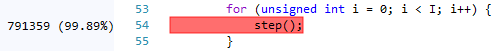
\includegraphics[width=0.7\textwidth]{images/hotpath_main.png}
  \caption{Hot path of \mintinline{c}{main()} function}
  \label{fig:hotpath_main}
\end{figure}

\begin{figure}[H]
  \centering
  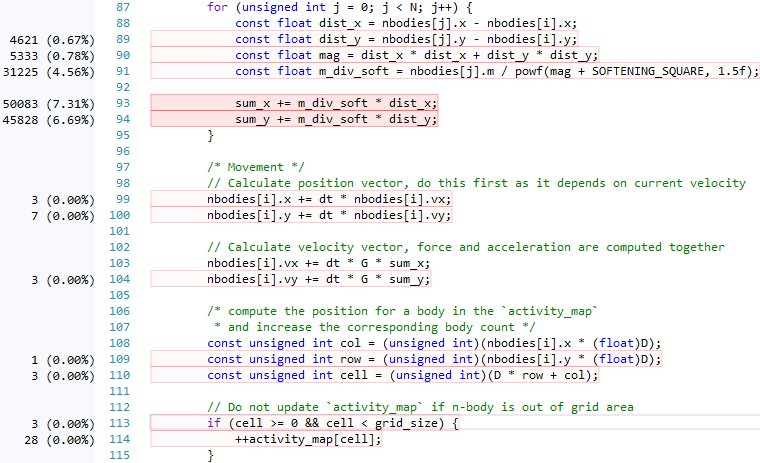
\includegraphics[width=0.97\textwidth]{images/hotpath_step.png}
  \caption{Hot path of \mintinline{c}{step()} function}
  \label{fig:hotpath_step}
\end{figure}

\subsubsection{Possible Optimisations for Serial Implementation} \label{subsec:serial_optimisation}
At line 91 of \cref{fig:hotpath_step}, it might be possible to reduce the computation cost of
\texttt{m\_div\_soft} by simplifying the equation. \texttt{m\_div\_soft} represents the following
part in \cref{equation:force},
\begin{equation*}
  \frac{m_j}{(||\vec{x_j} - \vec{x_i}||^2 + \epsilon^2)^\frac{3}{2}}
\end{equation*}
The denominator can be further simplified as follow,
\begin{equation*}
  \begin{aligned}
    (||\vec{x_j} - \vec{x_i}||^2 + \epsilon^2)^\frac{3}{2} &= \sqrt{(||\vec{x_j} - \vec{x_i}||^2 + \epsilon^2)^3} \\
    &= \sqrt{(||\vec{x_j} - \vec{x_i}||^2 + \epsilon^2)^2 \times (||\vec{x_j} - \vec{x_i}||^2 + \epsilon^2)} \\
    &= (||\vec{x_j} - \vec{x_i}||^2 + \epsilon^2)\sqrt{(||\vec{x_j} - \vec{x_i}||^2 + \epsilon^2)}
  \end{aligned}
\end{equation*}

Applying the modification to the code,
\begin{listing}[H]
  \begin{minted}[linenos, firstnumber=87, frame=lines, framesep=2mm, fontsize=\footnotesize]{c}
    for (unsigned int j = 0; j < N; j++) {
        ...
        const float mag_add_soft = dist_x * dist_x + dist_y * dist_y + SOFTENING_SQUARE;
        const float m_div_soft = nbodies[j].m / (mag_add_soft * sqrtf(mag_add_soft));
        ...
    }
  \end{minted}
  \caption{Attempt to optimise the \texttt{step()} function.}
  \label{listing:serial_optimisaton_attempt}
\end{listing}

\renewcommand{\arraystretch}{1.3}
\begin{longtable}{|c|c|c|c|}
  \hline \endfirsthead
  & \multicolumn{2}{c|}{Total Execution Time (seconds)} & \\ \cline{2-3}
  \multirow{-2}{*}{Number of Bodies (N)} & Before & After & \multirow{-2}{*}{Speedup} \\ \hline
  \rowcolor{lightgray}\multicolumn{4}{|c|}{\textbf{Number of Bodies (N)}} \\ \hline
  256  & 0.268 & 0.037 & 7.24 \\
  512  & 1.066 & 0.144 & 7.40 \\
  1024 & 4.264 & 0.569 & 7.49 \\
  2048 & 17.463 & 2.300 & 7.59 \\
  4096 & 68.358 & 9.353 & 7.31 \\ \hline
  \multicolumn{3}{|r|}{\textbf{Average}} & \textbf{7.406} \\ \hline
  \rowcolor{lightgray}\multicolumn{4}{|c|}{\textbf{Activity Grid Dimension (D)}} \\ \hline
  100   & 4.230 & 0.572 & 7.40\\
  1000  & 4.248 & 0.599 & 7.09 \\
  2000  & 4.402 & 0.736 & 5.98 \\
  5000  & 5.509 & 1.651 & 3.34 \\
  10000 & 8.477 & 5.020 & 1.69 \\ \hline
  \multicolumn{3}{|r|}{\textbf{Average}} & \textbf{5.1} \\ \hline
  \caption{Before and after the optimisation attempt of \cref{listing:serial_optimisaton_attempt} in iteration mode.}
  \label{table:serial_optimisation_attempt}
\end{longtable}
\renewcommand{\arraystretch}{1}

According to the results in \cref{table:serial_optimisation_attempt}, the optimisation attempt in
\cref{listing:serial_optimisaton_attempt} has improved the performance \textbf{significantly}. The
optimisation has achieved an average speedup of \textbf{7.406}. Moreover, the optimisation also
improves the performance in visualisation mode, as shown in \cref{fig:serial_optimisation_fps}.
Therfore, it is confirmed that the performance bottleneck was the \texttt{powf()} function.

\begin{figure}[h]
  \centering
  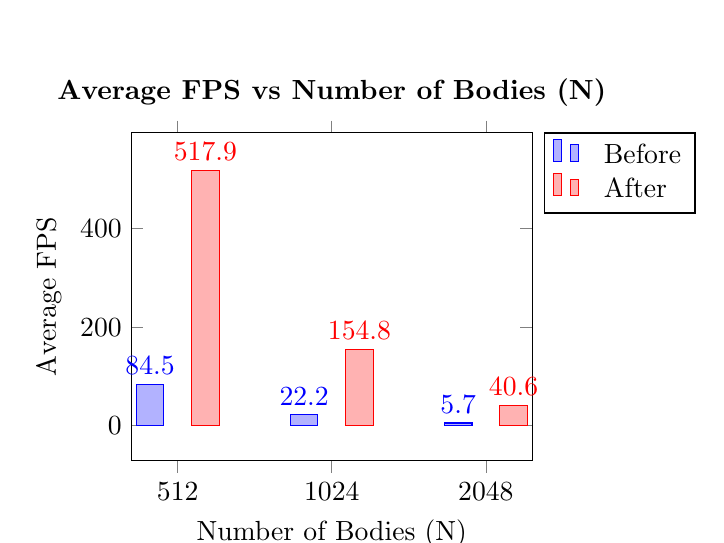
\begin{tikzpicture}
    \begin{axis}[
        width=0.55\textwidth,
        ybar=10pt,
        enlargelimits=0.15,
        legend cell align=left,
        legend style={column sep=7pt},
        legend pos=outer north east,
        title={\textbf{Average FPS vs Number of Bodies (N)}},
        xlabel=Number of Bodies (N), ylabel=Average FPS,
        symbolic x coords={512,1024,2048},
        xtick=data,
        nodes near coords,
      ]
      \addplot coordinates {(512,84.5) (1024,22.2) (2048,5.7)};
      \addplot coordinates {(512,517.9) (1024,154.8) (2048,40.6)};
      \legend{Before,After}
    \end{axis}
  \end{tikzpicture}
  \caption{Average FPS before and after the optimisation attempt of \cref{listing:serial_optimisaton_attempt}
    in visualisation mode (FPS recorded using CapFrameX \cite{capframex}).}
  \label{fig:serial_optimisation_fps}
\end{figure}

\subsubsection{Possible Optimisations for Parallel Implementation}
\begin{enumerate}
  \item For the \mintinline{c}{main()} function, the only possible optimisation is to parallelise the loop.

  \item For the \mintinline{c}{step()} function, the best candidate for optimisation is the summation
  calculation in the overall force ($F_i$) equation (line 89-90 in \cref{fig:hotpath_step}). There are
  three possible optimisation approaches for \mintinline{c}{step()} function:
  \begin{enumerate}
    \item Parallelise the outer loop (N-bodies loop)
    \item Parallelise the inner loop (Overall force \(F_i\) calculation loop)
    \item Parallelise both loops by nested parallelism
  \end{enumerate}
\end{enumerate}

\subsection{Benchmark Configuration}
To minimise the uncontrollable variables in the benchmark environment, all benchmarks are required
to be performed under the same configuration to improve consistency.

\subsubsection{Hardware Specifications} \label{subsec:hardware}
\begin{enumerate}
  \item Operating system: Windows 10 64-bit
  \item CPU: Intel\textsuperscript{\textregistered} Core\texttrademark\ i7-7700HQ, 4 cores, 8
  threads
  \item RAM: 16GB DDR4-2400MHz
\end{enumerate}

\subsubsection{Number of Simulation Iterations}
\textbf{Question:} Does the value of argument \textbf{I} affect the simulation performance?

Since \textbf{I} controls the number of simulations to run, then it is expected that the
total execution time would increase as \textbf{I} increases. A quick benchmark is conducted to
prove this hypothesis:

\textbf{Fixed arguments:} $\textbf{N} =$ 1000, $\textbf{D} =$ 10

\begin{figure}[ht]
  \centering
  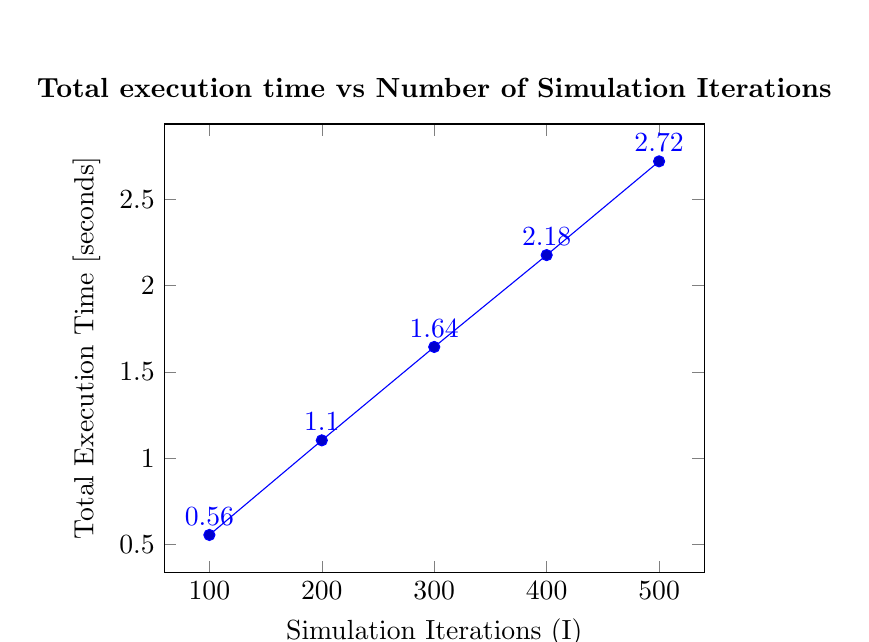
\begin{tikzpicture}
    \begin{axis}[
      nodes near coords,
      y unit=seconds,
      xlabel=Simulation Iterations (I), ylabel=Total Execution Time,
      title=\textbf{Total execution time vs Number of Simulation Iterations}]
      \addplot coordinates {
          (100, 0.555)
          (200, 1.103)
          (300, 1.644)
          (400, 2.176)
          (500, 2.719)
      };
    \end{axis}
  \end{tikzpicture}
  \caption{Relationship between the total execution time and number of simulation iterations.}
  \label{figure:simulation_iterations}
\end{figure}

According to \cref{figure:simulation_iterations}, the total execution time is \textbf{directly
proportional} to the number of simulation iterations. The value of \textbf{I} should only affect the
execution time proportionally, but not the simulation performance. Hence, it is decided to exclude
\textbf{I} from the benchmark variable.

\subsubsection{Number of Runs per Benchmark}
\noindent It is unlikely that the result of every same benchmark run is the same. There will be
minimal execution time difference between each run due to uncontrollable environment variables. This
can be mitigated by taking the average execution time of multiple benchmark runs to minimise the
error rate and randomness. Each benchmark result would be more accurate as well when compared to a
single benchmark run. \textbf{Conclusion:} It is decided to calculate the average execution time of
a single benchmark over 10 runs.

\subsection{Benchmark Results} \label{subsec:serial_results}
In this section, the benchmark results of serial implementation will be presented and commented.
These results act as a baseline to measure potential performance improvement in parallel version.

\subsubsection{Baseline Performance} \label{subsec:baseline}
The benchmark is done over a various values of \textbf{N} and \textbf{D} with the compute bound
optimisations applied.

\noindent\textcolor{red}{N.B.} The benchmarks are performed after the optimisation in
\cref{subsec:serial_optimisation}.

\subsubsection*{\underline{Benchmark on Number of Bodies (N)}}
\textbf{Fixed arguments:} $\textbf{D} =$ 10, $\textbf{I} =$ 100
\renewcommand{\arraystretch}{1.3}
\begin{longtable}{|c|c|c|}
  \hline \endfirsthead \rowcolor{lightgray}
  N    & Average Execution Time of 10 runs (seconds) \\ \hline
  256  & 0.037                                       \\
  512  & 0.144                                       \\
  1024 & 0.569                                       \\
  2048 & 2.300                                       \\
  4096 & 9.353                                       \\ \hline
  \caption{Baseline performance of program over various values of \textbf{N}.}
  \label{table:baseline_n}
\end{longtable}
\renewcommand{\arraystretch}{1}

\subsubsection*{\underline{Benchmark on Activity Grid Dimension (D)}}
\textbf{Fixed arguments:} $\textbf{N} =$ 1024, $\textbf{I} =$ 100
\renewcommand{\arraystretch}{1.3}
\begin{longtable}{|c|c|c|}
  \hline \endfirsthead \rowcolor{lightgray}
  D     & Average Execution Time of 10 runs (seconds) \\ \hline
  100   & 0.572                                       \\
  1000  & 0.599                                       \\
  2000  & 0.736                                       \\
  5000  & 1.651                                       \\
  10000 & 5.020                                       \\ \hline
  \caption{Baseline performance of program over various values of \textbf{D}.}
  \label{table:baseline_d}
\end{longtable}
\renewcommand{\arraystretch}{1}


\newpage
\section{Parallel Implementation} \label{sec:parallel_implementation}

\noindent\textcolor{red}{N.B.} All benchmarks follows the format and fixed arguments
used in the baseline performance benchmark (\cref{subsec:baseline}), where
\begin{itemize}
  \item \textbf{Fixed arguments:} $\textbf{D} =$ 10, $\textbf{I} =$ 100 for benchmarks on \textbf{N}
  \item \textbf{Fixed arguments:} $\textbf{N} =$ 1024, $\textbf{I} =$ 100 for benchmarks on \textbf{D}
\end{itemize}

\textbf{Section 4.1 to 4.4} aims to assess the effectiveness of each parallelisation strategy by
parallelising one loop at a time in \textbf{iteration mode}. Scheduling types and chunk sizes are
also included in the benchmarks for each parallelisation strategy.

\subsection{\texttt{main()}: Simulation Iterations Loop} \label{subsec:iter_loop}

\begin{listing}[H]
  \begin{minted}[linenos, frame=lines, framesep=2mm, fontsize=\footnotesize]{c}
  int main(const int argc, char *argv[]) {
      ...
      // This do not ensure correctness, justification below
  #pragma omp parallel for default(none) shared(N, D)
      for (i = 0; i < (int)I; i++) {
          step();
      }
      ...
  }
  \end{minted}
  \caption{Parallelising the simulation iterations loop in \texttt{main()} function.}
  \label{listing:iter_loop}
\end{listing}

Parallelising the simulation iterations is not a good approach. This is because:
\begin{enumerate}
  \item Each thread must have its own instance of \texttt{nbodies} and \texttt{activity\_map} to
  prevent race conditions from occuring within the \texttt{step()} function.
  \item Each step is dependent on the previous step (see \cref{subsec:calculate_movement}). This
  implies that an \texttt{ordered} clause needs to added to the \texttt{parallel for} construct to
  execute the \texttt{step()} function call  in serial, which is equivalent to executing the loop
  in serial.
  \item The simulation iterations loop will only be executed in iteration mode. Therefore, it will
  not have any impact on the performance of visualisation mode.
\end{enumerate}

\newpage
\subsection{\texttt{step()}: Outer N-Bodies Loop} \label{subsec:nbody_loop}
\begin{listing}[ht]
  \begin{minted}[linenos, frame=lines, framesep=2mm, fontsize=\footnotesize]{c}
  static void step(void) {
  #pragma omp parallel for default(none) shared(N, D, nbodies, activity_map) if (M == OPENMP)
      for (i = 0; i < (int)N; i++) {
        ...
        if (cell >= 0 && cell < grid_size) {
            // Race condition for `activity_map`
            ++activity_map[cell];
        }
      }
  }
  \end{minted}
  \caption{Parallelising the outer N-bodies loop in \texttt{step()} function.}
  \label{listing:nbody_loop}
\end{listing}

\subsubsection{Race Condition Synchronisation}
\renewcommand{\arraystretch}{1.3}
\begin{longtable}{|c|c|c|c|}
  \hline \endfirsthead
  & & \multicolumn{2}{c|}{Synchronisation (seconds)} \\ \cline{3-4}
  \multirow{-2}{*}{Value} & \multirow{-2}{*}{Baseline (seconds)}
  & critical & atomic \\ \hline
  \rowcolor{lightgray} \multicolumn{4}{|c|}{\textbf{Number of Bodies (N)}} \\ \hline
  256  & 0.037 & 0.013 & \cellcolor{green}0.012 \\
  512  & 0.144 & \cellcolor{green}0.042 & 0.044 \\
  1024 & 0.569 & \cellcolor{green}0.152 & \cellcolor{green}0.152 \\
  2048 & 2.300 & 0.628 & \cellcolor{green}0.594 \\
  4096 & 9.353 & 2.457 & \cellcolor{green}2.303 \\
  \rowcolor{lightgray} \multicolumn{4}{|c|}{\textbf{Activity Grid Dimension (D)}} \\ \hline
  100   & 0.572 & 0.157 & \cellcolor{green}0.155 \\
  1000  & 0.599 & 0.182 & \cellcolor{green}0.178 \\
  2000  & 0.736 & 0.345 & \cellcolor{green}0.329 \\
  5000  & 1.651 & 1.388 & \cellcolor{green}1.321 \\
  10000 & 5.020 & 5.005 & \cellcolor{green}4.984 \\ \hline
  \caption{Benchmark of synchronisation techniques for \texttt{activity\_map} race condition.}
  \label{table:step_outer_race}
\end{longtable}
\renewcommand{\arraystretch}{1}

The results in \cref{table:step_outer_race} have shown that both \texttt{omp critical} and
\texttt{omp atomic} perform better than the baseline performance, and \texttt{omp atomic} performs
faster than \texttt{omp critical}. \textcolor{red}{N.B.} Hence, \texttt{omp atomic} is a better
approach for avoiding the race condition.

\noindent\underline{\textbf{Question:} Can \mintinline{c}{omp master} and a local activity map prevent the race condition?}

No. To prevent the race condition using \texttt{omp master} and a local activity map, the local
activity map must be a 2D array. However, the dimension \textbf{D} is only known at runtime and it
is not a constant. The compiler will generate compile error C2057 \cite{c2057} for declaring the 2D
array with unknown size at compile time, such as \mintinline{c}{float local_activity_map[D * D][N]}.

\subsubsection{Static Scheduling} \label{subsec:nbody_loop_static}
\renewcommand{\arraystretch}{1.3}
\begin{longtable}{|c|c|c|c|c|c|c|}
  \hline \endfirsthead
  & & \multicolumn{5}{c|}{Chunk Size (seconds)} \\ \cline{3-7}
  \multirow{-2}{*}{Value} & \multirow{-2}{*}{Baseline (seconds)}
  & default & 1 & 2 & 4 & 8 \\ \hline
  \rowcolor{lightgray} \multicolumn{7}{|c|}{\textbf{Number of Bodies (N)}} \\ \hline
  256  & 0.037 & \cellcolor{green} 0.011 & 0.013 & 0.012 & 0.014 & 0.014 \\
  512  & 0.144 & \cellcolor{green}0.040 & 0.041 & 0.043 & 0.071 & 0.046 \\
  1024 & 0.569 & \cellcolor{green}0.158 & 0.160 & 0.162 & 0.182 & 0.160 \\
  2048 & 2.300 & \cellcolor{green}0.611 & 0.622 & 0.607 & 0.607 & 0.608 \\
  4096 & 9.353 & \cellcolor{green}2.343 & 2.494 & 2.470 & 2.441 & 2.383 \\ \hline
  \rowcolor{lightgray} \multicolumn{7}{|c|}{\textbf{Activity Grid Dimension (D)}} \\ \hline
  100   & 0.572 & \cellcolor{green}0.156 & 0.186 & 0.167 & 0.158 & 0.159 \\
  1000  & 0.599 & \cellcolor{green}0.176 & 0.182 & 0.184 & 0.196 & 0.199 \\
  2000  & 0.736 & 0.343 & 0.378 & 0.377 & 0.337 & \cellcolor{green}0.335 \\
  5000  & 1.651 & \cellcolor{green}1.377 & 1.420 & 1.396 & 1.427 & 1.387 \\
  10000 & 5.020 & 4.972 & 5.017 & \cellcolor{green}4.933 & 4.934 & 4.942 \\ \hline
  \caption{Benchmark of parallelising outer N-bodies loop with static scheduling.}
  \label{table:nbody_loop_static}
\end{longtable}
\renewcommand{\arraystretch}{1}

The results in \cref{table:nbody_loop_static} have shown that the default chunk size (determined by
OpenMP) has the best overall performance improvements. This indicates that the workloads are equally
shared between each thread.

\subsubsection{Dynamic Scheduling} \label{subsec:nbody_loop_dynamic}
\renewcommand{\arraystretch}{1.3}
\begin{longtable}{|c|c|c|c|c|c|}
  \hline \endfirsthead
  & & \multicolumn{4}{c|}{Chunk Size (seconds)} \\ \cline{3-6}
  \multirow{-2}{*}{Value} & \multirow{-2}{*}{Baseline (seconds)}
  & 1 (default) & 2 & 4 & 8 \\ \hline
  \rowcolor{lightgray} \multicolumn{6}{|c|}{\textbf{Number of Bodies (N)}} \\ \hline
  256  & 0.037 & 0.015 & 0.013 & \cellcolor{green}0.012 & 0.013 \\
  512  & 0.144 & 0.045 & \cellcolor{green}0.042 & 0.045 & \cellcolor{green}0.042 \\
  1024 & 0.569 & \cellcolor{green}0.156 & 0.159 & \cellcolor{green}0.156 & 0.160 \\
  2048 & 2.300 & 0.592 & 0.590 & \cellcolor{green}0.588 & 0.594 \\
  4096 & 9.353 & \cellcolor{green}2.309 & 2.329 & 2.314 & 2.330 \\ \hline
  \rowcolor{lightgray} \multicolumn{6}{|c|}{\textbf{Activity Grid Dimension (D)}} \\ \hline
  100   & 0.572 & \cellcolor{green}0.157 & 0.173 & 0.158 & 0.159 \\
  1000  & 0.599 & 0.188 & 0.190 & \cellcolor{green}0.181 & 0.180 \\
  2000  & 0.736 & 0.346 & 0.409 & 0.339 & \cellcolor{green}0.338 \\
  5000  & 1.651 & 1.390 & \cellcolor{green}1.368 & 1.391 & 1.383 \\
  10000 & 5.020 & 4.991 & 4.959 & \cellcolor{green}4.909 & 4.936 \\ \hline
  \caption{Benchmark of parallelising outer N-bodies loop with dynamic scheduling.}
  \label{table:nbody_loop_dynamic}
\end{longtable}
\renewcommand{\arraystretch}{1}

The best chunk size could not be deduced based on the results in \cref{table:nbody_loop_dynamic}.
Dynamic scheduling produces inconsistent results, and thus is not suitable for this parallelisation
strategy.

\subsubsection{Performance Improvements}
Based on the benchmark results and analysis in
\cref{subsec:nbody_loop_static,subsec:nbody_loop_dynamic}, static scheduling with default chunk size
is selected as the scheduling type for this parallelisation strategy.

\noindent Average performance speedup for \textbf{Number of Bodies (N)} with
\textcolor{blue}{\texttt{schedule(static)}}:

\(\cfrac{\dfrac{0.037}{0.011} + \dfrac{0.144}{0.040} + \dfrac{0.569}{0.158} + \dfrac{2.300}{0.611} + \dfrac{9.353}{2.343}}{5} = 3.45\)

\noindent Average performance speedup for \textbf{Activity Grid Dimension (D)}
\textcolor{blue}{\texttt{schedule(static)}}:

\(\cfrac{\dfrac{0.572}{0.156} + \dfrac{0.599}{0.176} + \dfrac{0.736}{0.343} + \dfrac{1.651}{1.377} + \dfrac{5.020}{4.972}}{5} = 2.28\)


\newpage
\subsection{\texttt{step()}: Inner Overall Force \texorpdfstring{$(F_i)$}~ Calculation Loop}
\label{subsec:force_loop}
\begin{listing}[ht]
  \begin{minted}[linenos, frame=lines, framesep=2mm, fontsize=\footnotesize]{c}
  static void step(void) {
      ...
      for (i = 0; i < (int)N; i++) {
          float sum_x = 0, sum_y = 0;

  #pragma omp parallel for default(none) shared(N) if (M == OPENMP)
          for (j = 0; j < (int)N; j++) {
              ...
              // Race condition below
              sum_x += m_div_soft * dist_x;
              sum_y += m_div_soft * dist_y;
          }
      }
      ...
  }
  \end{minted}
  \caption{Parallelising the inner loop in \texttt{step()} function.}
\end{listing}

\subsubsection{Race Condition Synchronisation}
\renewcommand{\arraystretch}{1.3}
\begin{longtable}{|c|c|c|c|c|}
  \hline \endfirsthead \rowcolor{lightgray}
  & & \multicolumn{3}{c|}{Synchronisation (seconds)} \\ \cline{3-5}
  \multirow{-2}{*}{\cellcolor{lightgray}Number of Bodies (N)} &
  \multirow{-2}{*}{\cellcolor{lightgray}Baseline (seconds)}
  & critical & atomic & reduction \\ \hline
  256  & \cellcolor{green}0.037 & 0.822 & 0.722 & 0.049 \\
  512  & 0.144 & 3.275 & 3.271 & \cellcolor{green}0.114 \\
  1024 & 0.569 & 12.892 & 14.319 & \cellcolor{green}0.297 \\
  2048 & 2.300 & 51.49 & 54.137 & \cellcolor{green}0.879 \\
  4096 & 9.353 & 278.471 & 229.10 & \cellcolor{green}2.911 \\ \hline
  \caption{Benchmark of synchronisation techniques for \texttt{sum\_x}, \texttt{sum\_y} race condition.}
  \label{table:step_inner_race}
\end{longtable}
\renewcommand{\arraystretch}{1}

\cref{table:step_inner_race} has shown that \texttt{reduction} outperforms \texttt{omp critical} and
\texttt{omp atomic}. Therefore, \texttt{reduction} will be used to avoid the race conditions for
\texttt{sum\_x} and \texttt{sum\_y}.

\subsubsection{Static Scheduling} \label{subsec:force_loop_static}
\renewcommand{\arraystretch}{1.3}
\begin{longtable}{|c|c|c|c|c|c|c|}
  \hline \endfirsthead
  & & \multicolumn{5}{c|}{Chunk Size (seconds)} \\ \cline{3-7}
  \multirow{-2}{*}{Value} & \multirow{-2}{*}{Baseline (seconds)}
  & default & 1 & 2 & 4 & 8 \\ \hline
  \rowcolor{lightgray} \multicolumn{7}{|c|}{\textbf{Number of Bodies (N)}} \\ \hline
  256  & \cellcolor{green}0.037 & 0.048 & 0.048 & 0.052 & 0.050 & 0.050 \\
  512  & 0.144 & \cellcolor{green}0.111 & 0.117 & 0.117 & 0.117 & 0.118 \\
  1024 & 0.569 & \cellcolor{green}0.296 & 0.319 & 0.349 & 0.334 & 0.322 \\
  2048 & 2.300 & \cellcolor{green}0.874 & 0.975 & 1.018 & 1.004 & 1.000 \\
  4096 & 9.353 & \cellcolor{green}2.942 & 3.174 & 3.604 & 3.303 & 3.195 \\ \hline
  \rowcolor{lightgray} \multicolumn{7}{|c|}{\textbf{Activity Grid Dimension (D)}} \\ \hline
  100   & 0.572 & \cellcolor{green}0.293 & 0.453 & 0.323 & 0.312 & 0.306 \\
  1000  & 0.599 & \cellcolor{green}0.328 & 0.365 & 0.390 & 0.385 & 0.372 \\
  2000  & 0.736 & \cellcolor{green}0.483 & 0.531 & 0.545 & 0.526 & 0.517 \\
  5000  & 1.651 & \cellcolor{green}1.466 & 1.558 & 1.559 & 1.544 & 1.548 \\
  10000 & \cellcolor{green}5.020 & 5.060 & 5.171 & 5.150 & 5.103 & 5.119 \\ \hline
  \caption{Benchmark of parallelising inner force calculation loop with static scheduling.}
  \label{table:force_loop}
\end{longtable}
\renewcommand{\arraystretch}{1}

The results in \cref{table:force_loop} have shown that the default chunk size has the best overall
performance improvements. This indicates that the workloads are equally shared between each thread.

The benchmark where \(\textbf{N} =\) 256 shows that the baseline performance is faster than the
parallelised performance. This is possible as there is some overhead in forking/joining of threads,
and the overhead added is larger than the performance improvements achieved. Hence, if the value of
\textbf{N} is small, it is better to execute the loop in serial.

\subsubsection{Dynamic Scheduling} \label{subsec:force_loop_dynamic}
\renewcommand{\arraystretch}{1.3}
\begin{longtable}{|c|c|c|c|c|c|c|c|}
  \hline \endfirsthead
  & & \multicolumn{6}{c|}{Chunk Size (seconds)} \\ \cline{3-8}
  \multirow{-2}{*}{Value} & \multirow{-2}{*}{Baseline (seconds)}
  & 1 (default) & 2 & 4 & 8 & 32 & 64 \\ \hline
  \rowcolor{lightgray} \multicolumn{8}{|c|}{\textbf{Number of Bodies (N)}} \\ \hline
  256  & \cellcolor{green}0.037 & 0.718  & 0.453  & 0.310  & 0.307 & 0.292 & 0.282 \\
  512  & \cellcolor{green}0.144 & 1.886  & 1.498  & 1.250  & 0.699 & 0.602 & 0.587 \\
  1024 & \cellcolor{green}0.569 & 6.877  & 4.809  & 3.392  & 2.817 & 1.271 & 1.244 \\
  2048 & \cellcolor{green}2.300 & 25.224 & 15.580 & 12.094 & 7.881 & 4.287 & 3.087 \\
  4096 & \cellcolor{green}9.353 & 83.913 & 56.561 & 40.620 & 26.950 & 11.991 & 10.290 \\ \hline
  \rowcolor{lightgray} \multicolumn{8}{|c|}{\textbf{Activity Grid Dimension (D)}} \\ \hline
  100   & \cellcolor{green}0.572 & 6.543  & 4.571 & 3.254 & 2.861 & 1.283 & 1.243 \\
  1000  & \cellcolor{green}0.599 & 6.451  & 4.631 & 3.336 & 2.880 & 1.317 & 1.283 \\
  2000  & \cellcolor{green}0.736 & 6.610  & 4.767 & 3.505 & 3.029 & 1.488 & 1.450 \\
  5000  & \cellcolor{green}1.651 & 8.036  & 5.773 & 4.485 & 4.005 & 2.493 & 2.436 \\
  10000 & \cellcolor{green}5.020 & 11.364 & 9.273 & 7.983 & 7.659 & 6.030 & 5.998 \\ \hline
  \caption{Benchmark of parallelising inner force calculation loop with dynamic scheduling.}
  \label{table:force_loop_dynamic}
\end{longtable}
\renewcommand{\arraystretch}{1}

As shown in \cref{table:force_loop_dynamic}, dynamic scheduling has caused the execution time to
increase. Although the increase in execution time is lower with larger chunk sizes, it is still
slower than the baseline performance. Hence, dynamic scheduling is not applicable for this
parallelisation strategy.

\subsubsection{Performance Improvements}
Based on the benchmark results and analysis in
\cref{subsec:force_loop_static,subsec:force_loop_dynamic}, static scheduling with default chunk size
is selected as the scheduling type for this parallelisation strategy.

\noindent Average performance speedup for \textbf{Number of Bodies (N)} with \textcolor{blue}{\texttt{schedule(static)}}:

\(\cfrac{\dfrac{0.037}{0.048} + \dfrac{0.144}{0.111} + \dfrac{0.569}{0.296} + \dfrac{2.300}{0.874} + \dfrac{9.353}{2.942}}{5} = 2.06\)

\noindent Average performance speedup for \textbf{Activity Grid Dimension (N)} with \textcolor{blue}{\texttt{schedule(static)}}:

\(\cfrac{\dfrac{0.572}{0.293} + \dfrac{0.599}{0.328} + \dfrac{0.736}{0.483} + \dfrac{1.651}{1.466} + \dfrac{5.020}{5.060}}{5} = 1.48\)

\newpage
\subsection{\texttt{step()}: Activity Map Normalisation Loop} \label{subsec:map_loop}
\begin{listing}[H]
  \begin{minted}[linenos, frame=lines, framesep=2mm, fontsize=\footnotesize]{c}
  static void step(void) {
      ...
      const float normalise = (float)D / (float)N;
  #pragma omp parallel for shared(activity_map) if (M == OPENMP)
      for (i = 0; i < (int)grid_size; ++i) {
          activity_map[i] *= normalise;
      }
  }
  \end{minted}
  \caption{Parallelising the activity map normalisation loop in \texttt{step()} function.}
\end{listing}

\subsubsection{Static Scheduling}
\renewcommand{\arraystretch}{1.3}
\begin{longtable}{|c|c|c|c|c|c|c|}
  \hline \endfirsthead
  & & \multicolumn{5}{c|}{Chunk Size (seconds)} \\
  \cline{3-7}
  \multirow{-2}{*}{Value} & \multirow{-2}{*}{Baseline (seconds)}
  & default & 1 & 2 & 4 & 8 \\ \hline
  \rowcolor{lightgray} \multicolumn{7}{|c|}{\textbf{Number of Bodies (N)}} \\ \hline
  256  & \cellcolor{green}0.037 & 0.066 & 0.066 & 0.066 & 0.066 & 0.067 \\
  512  & \cellcolor{green}0.144 & 0.264 & 0.263 & 0.263 & 0.264 & 0.263 \\
  1024 & \cellcolor{green}0.569 & 1.054 & 1.055 & 1.056 & 1.062 & 1.053 \\
  2048 & \cellcolor{green}2.300 & 4.213 & 4.215 & 4.209 & 4.229 & 4.216 \\
  4096 & \cellcolor{green}9.353 & 14.052 & 14.102 & 14.083 & 14.119 & 14.142 \\ \hline
  \rowcolor{lightgray} \multicolumn{7}{|c|}{\textbf{Activity Grid Dimension (D)}} \\ \hline
  100   & \cellcolor{green}0.572 & 1.052 & 1.054 & 1.053 & 1.053 & 1.053 \\
  1000  & \cellcolor{green}0.599 & 1.090 & 1.114 & 1.103 & 1.105 & 1.096 \\
  2000  & \cellcolor{green}0.736 & 1.240 & 1.316 & 1.283 & 1.293 & 1.297 \\
  5000  & \cellcolor{green}1.651 & 2.312 & 2.875 & 2.524 & 2.589 & 2.642 \\
  10000 & \cellcolor{green}5.020 & 5.924 & 9.854 & 8.617 & 8.450 & 7.338 \\ \hline
  \caption{Benchmark of parallelising activity map loop with static scheduling.}
  \label{table:step_activity_static}
\end{longtable}
\renewcommand{\arraystretch}{1}

\subsubsection{Dynamic Scheduling}
\renewcommand{\arraystretch}{1.3}
\begin{longtable}{|c|c|c|c|c|c|}
  \hline \endfirsthead
  & & \multicolumn{4}{c|}{Chunk Size (seconds)} \\
  \cline{3-6}
  \multirow{-2}{*}{Value} & \multirow{-2}{*}{Baseline (seconds)}
  & 1 (default) & 2 & 4 & 8 \\ \hline
  \rowcolor{lightgray} \multicolumn{6}{|c|}{\textbf{Number of Bodies (N)}} \\ \hline
  256  & \cellcolor{green}0.037 & 0.067 & 0.067 & 0.067 & 0.067 \\
  512  & \cellcolor{green}0.144 & 0.264 & 0.265 & 0.267 & 0.264 \\
  1024 & \cellcolor{green}0.569 & 1.054 & 1.053 & 1.059 & 1.055 \\
  2048 & \cellcolor{green}2.300 & 4.222 & 4.215 & 4.242 & 4.218 \\
  4096 & \cellcolor{green}9.353 & 14.128 & 14.128 & 14.72 & 14.158 \\ \hline
  \rowcolor{lightgray} \multicolumn{6}{|c|}{\textbf{Activity Grid Dimension (D)}} \\ \hline
  100   & \cellcolor{green}0.572 & 1.085 & 1.070 & 1.062 & 1.080 \\
  1000  & \cellcolor{green}0.599 & 3.871 & 2.485 & 1.808 & 1.467 \\
  2000  & \cellcolor{green}0.736 & 11.819 & 6.787 & 4.032 & 2.677 \\
  5000  & \cellcolor{green}1.651 & 70.271 & 37.69 & 19.927 & 11.326 \\
  10000 & \cellcolor{green}5.020 & 274.31 & 144.390 & 76.251 & 41.420 \\ \hline
  \caption{Benchmark of parallelising activity map loop with dynamic scheduling.}
  \label{table:step_activity_dynamic}
\end{longtable}
\renewcommand{\arraystretch}{1}

\subsubsection{Performance Improvements}
No performance improvements have been observed in
\cref{table:step_activity_static,table:step_activity_dynamic}. Conversely, parallelising the
activity map normalisation loop has an adverse effect on performance. Since the loop only has a
single multiplication operation, the performance improvements might not be sufficient to cover the
forking/joining overhead of threads. \textcolor{red}{N.B.} Therefore, the activity map normalisation
loop is already in optimal condition and does not require any further modification.

\subsection{Parallel Nesting Analysis} \label{subsec:nesting}
This section aims to investigate the possibility to further improve the performance through nested
parallelism.

\subsubsection{Outer N-bodies Loop + Inner Overall Force Calculation Loop}

\renewcommand{\arraystretch}{1.3}
\begin{longtable}{|c|c|c|c|}
  \hline \endfirsthead
  \multirow{2}{*}{Value} & \multirow{2}{*}{Baseline (seconds)} & Outer N-bodies & \multirow{2}{*}{Speedup} \\
  & & + Inner Force Calculation (seconds) & \\ \hline
  \rowcolor{lightgray} \multicolumn{4}{|c|}{\textbf{Number of Bodies (N)}} \\ \hline
  256  & \cellcolor{green}0.037 & 0.321 & 0.12 \\
  512  & \cellcolor{green}0.144 & 0.388 & 0.37 \\
  1024 & \cellcolor{green}0.569 & 0.594 & 0.96 \\
  2048 & 2.300 & \cellcolor{green}1.172 & 1.96 \\
  4096 & 9.353 & \cellcolor{green}3.350 & 2.79 \\ \hline
  \multicolumn{3}{|r|}{\textbf{Average}} & \textbf{1.24} \\ \hline
  \rowcolor{lightgray} \multicolumn{4}{|c|}{\textbf{Activity Grid Dimension (D)}} \\ \hline
  100   & \cellcolor{green}0.572 & 0.640 & 0.89 \\
  1000  & \cellcolor{green}0.599 & 0.615 & 0.97 \\
  2000  & \cellcolor{green}0.736 & 0.817 & 0.90 \\
  5000  & \cellcolor{green}1.651 & 1.854 & 0.89 \\
  10000 & \cellcolor{green}5.020 & 5.511 & 0.91 \\ \hline
  \multicolumn{3}{|r|}{\textbf{Average}} & \textbf{0.91} \\ \hline
  \caption{Parallelising both outer N-bodies and inner force calculation loop.}
\end{longtable}
\renewcommand{\arraystretch}{1}

The performance speedup achieved by parallel nesting is poor in comparison with the parallelisation
strategy in \cref{subsec:nbody_loop,subsec:force_loop}. Possible reasons are listed as follow:
\begin{enumerate}
  \item Parallel nesting may create too many threads and cause thread oversubscription
  \cite{nested_parallelism_tips}, where the number of simultaneously working threads are more than
  the number of available logical cores on the system. This can cause performance issues as the
  CPU would spend more time switching between tasks (context switching)
  \cite{thread_oversubscription}.
  \item The extra overhead added for additional forking/joining of threads in the nested parallel
  region. If the performance improvements are not sufficient to cover the extra overhead, then the
  overall performance will decrease.
\end{enumerate}


\subsection{Summary} \label{subsec:benchmark_summary}
Summarising the performance improvements achieved in iteration mode by each parallelisation strategy:
\begin{enumerate}
  \item \texttt{step()}: Outer N-bodies Loop, (static, default chunk).
    \begin{itemize}
      \item Average speedup for \textbf{N}: 3.54
      \item Average speedup for \textbf{D}: 2.28
    \end{itemize}
  \item \texttt{step()}: Inner Overall Force ($F_i$) Calculation Loop, (static, default chunk)
    \begin{itemize}
      \item Average speedup for \textbf{N}: 2.06
      \item Average speedup for \textbf{D}: 1.48
    \end{itemize}
  \item \texttt{step()}: Outer N-bodies + Inner Overall Force ($F_i$) Calculation Loop
    \begin{itemize}
      \item Average speedup for \textbf{N}: 1.24
      \item Average speedup for \textbf{D}: 0.91
    \end{itemize}
\end{enumerate}

The result above has shown that \textbf{parallelising the outer N-bodies loop} is the optimal strategy.

\newpage
\section{Visualisation Performance Improvements} \label{sec:visualisation_performance}
All benchmarks in the previous sections are being carried out in iteration mode to measure and
compare the performance of the program over large simulations. This sections aims to compare the
visualisation performance improvements between the serial and parallel implementation.

\begin{figure}[ht]
  \centering
  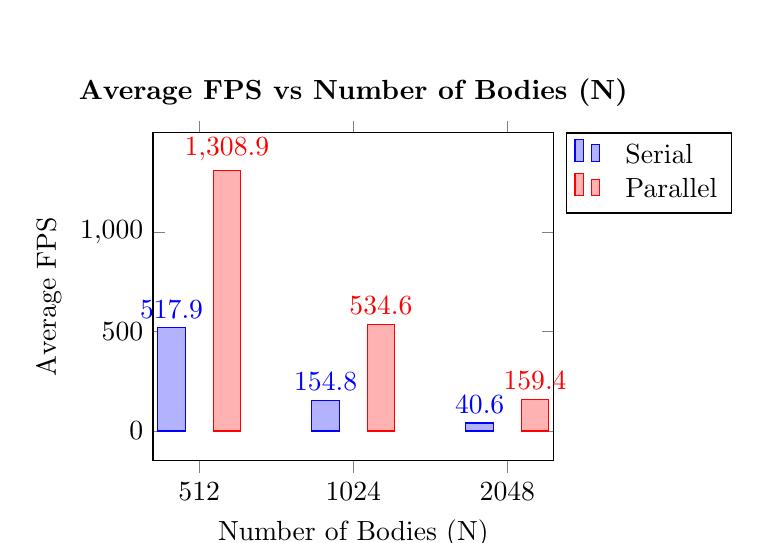
\begin{tikzpicture}
    \begin{axis}[
        width=0.55\textwidth,
        ybar=10pt,
        enlargelimits=0.15,
        legend cell align=left,
        legend style={column sep=7pt},
        legend pos=outer north east,
        title={\textbf{Average FPS vs Number of Bodies (N)}},
        xlabel=Number of Bodies (N), ylabel=Average FPS,
        symbolic x coords={512,1024,2048},
        xtick=data,
        nodes near coords,
      ]
      \addplot coordinates {(512,517.9) (1024,154.8) (2048,40.6)};
      \addplot coordinates {(512,1308.9) (1024,534.6) (2048,159.4)};
      \legend{Serial,Parallel}
    \end{axis}
  \end{tikzpicture}
  \caption{Comparison between the average FPS of serial and parallel implementation in visualisation mode.}
  \label{fig:average_fps_comparison}
\end{figure}

As shown in \cref{fig:average_fps_comparison}, parallelising the outer N-bodies loop will increase
the performance in visualisation mode as well.

\begin{figure}[H]
  \centering
  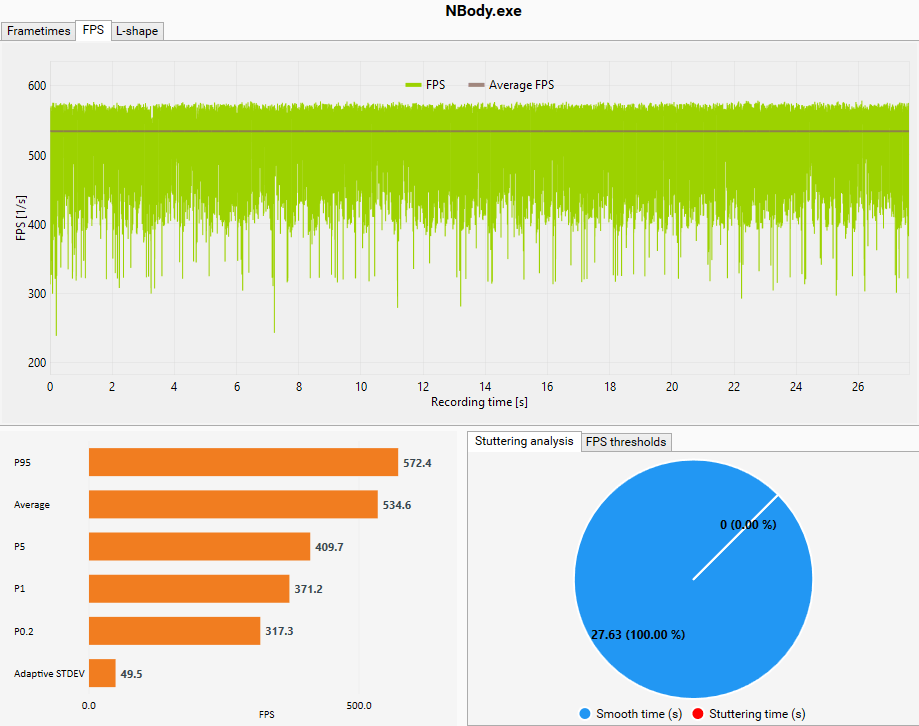
\includegraphics[width=0.7\textwidth]{images/capframex.png}
  \caption{Interface of CapFrameX \cite{capframex}, a free software for FPS monitoring.}
\end{figure}

\printbibliography

\end{document}
